% ---------------------------------------------------------------------------
% IT5006 Fundamentals of Data Analytics
% Group Project Milestone 1: Literature Review and Exploratory Data Analysis
%
% Compiles with pdfLaTeX. Build: pdflatex -> bibtex -> pdflatex x2
% ---------------------------------------------------------------------------
\documentclass[11pt,a4paper]{article}

\usepackage{lmodern}      % scalable Type 1 font; required for microtype expansion
\usepackage[T1]{fontenc}
\usepackage[utf8]{inputenc}
\usepackage[margin=1in]{geometry}
\usepackage{graphicx}
\usepackage{booktabs}
\usepackage{caption}
\usepackage{subcaption}
\usepackage{amsmath}
\usepackage{tikz}
\usetikzlibrary{arrows.meta,positioning}
\usepackage{microtype}
\usepackage{xcolor}
\usepackage[numbers,sort&compress]{natbib}
\usepackage[hidelinks]{hyperref}

\graphicspath{{figures/}}
\captionsetup{font=small,labelfont=bf,skip=5pt}
\setlength{\parskip}{0.18em}
\setlength{\textfloatsep}{10pt plus 2pt minus 2pt}
\setlength{\intextsep}{10pt plus 2pt minus 2pt}
\bibliographystyle{plainnat}

% Footnotes lettered, with a visible rule, so the notes read as marginal
% commentary rather than as numbered citations.
\renewcommand{\thefootnote}{\alph{footnote}}
\renewcommand{\footnoterule}{\vspace*{4pt}\hrule width 0.45\columnwidth height 0.4pt\vspace*{4pt}}
\makeatletter
\renewcommand\@makefntext[1]{\parindent 1em\noindent\hb@xt@1.4em{\hss\@makefnmark}\footnotesize #1}
\makeatother

% Citation marks a little smaller than body text.
\let\oldcitep\citep
\renewcommand{\citep}[1]{{\footnotesize\oldcitep{#1}}}
\let\oldcitet\citet
\renewcommand{\citet}[1]{{\footnotesize\oldcitet{#1}}}

\newcommand{\code}[1]{\texttt{\small #1}}

% ---------------------------------------------------------------------------
\begin{document}

% ============================== COVER PAGE =================================
\begin{titlepage}
\centering
\vspace*{3.5cm}

{\Large\bfseries Group Project Milestone 1:\par}
\vspace{0.6em}
{\Large\bfseries Literature Review and Exploratory Data Analysis\par}

\vspace{1.2cm}
{\large Predicting Delivery Performance and Customer Satisfaction\par}
\vspace{0.4em}
{\normalsize An analysis of 99{,}441 orders from the Olist Brazilian e-commerce marketplace\par}

\vspace{3.5cm}

{\large\bfseries Group 10\par}
\vspace{0.9em}

{\normalsize
\begin{tabular}{@{}l@{\hspace{1.5em}}l@{}}
Pan Pinyou  & A0329105L \\[3pt]
Li Yudan    & A0330335R \\[3pt]
Zhu Gengyu  & A0333773Y \\
\end{tabular}\par}

\vfill

{\large National University of Singapore\par}
\vspace{0.4em}
{\large IT5006 Fundamentals of Data Analytics\par}
\vspace{0.4em}
{\large AY2026/2027 Semester 1\par}

\vspace{1.1cm}
{\normalsize
\textbf{Dashboard:} \url{https://it5006-group-project-10.streamlit.app}\\[4pt]
\textbf{Repository:} \url{https://github.com/gengyuzhu/IT5006-Group-Project-10}\par}

\vspace{1.2cm}
\end{titlepage}

% ============================== BODY =======================================
\section{Literature Review}

\subsection{Scope}

This project analyses the \emph{Olist Brazilian E-Commerce} dataset: nine
relational tables covering 99{,}441 orders placed on a Brazilian marketplace
between September 2016 and October 2018 \citep{olist2018dataset}. Olist aggregates
small sellers onto Brazil's large retail platforms and handles fulfilment, so each
order links a customer, one or more sellers, a basket, a payment, a delivery and
usually a review -- a structure supporting all three question families the brief
identifies: operational performance, customer experience and commercial outcomes.
The review below covers what Phase 2 depends on: fulfilment and satisfaction,
model families for tabular data, feature engineering on a relational order model,
and metrics that survive severe imbalance.

\subsection{Fulfilment, delivery promises and customer satisfaction}

The e-commerce service-quality literature is unusually direct about which lever
matters. \citet{parasuraman2005esqual} decompose electronic service quality into
efficiency, \emph{fulfilment}, system availability and privacy, and find
fulfilment -- the accuracy of delivery promises and the condition in which goods
arrive -- among the strongest contributors to perceived quality.
\citet{rao2011elsq} sharpen this into logistics terms across 260 online retailers.
Transactional evidence at platform scale now confirms it: across more than 15
million marketplace orders, \citet{deshpande2023logistics} trace a chain rather
than a single link -- logistics performance drives the service rating a customer
leaves, and that rating in turn moves seller sales. That chain makes a low-review
model a commercial instrument rather than a diagnostic.

The promise itself is a second, less obvious decision variable.
\citet{cui2024promise} show that committing to a faster delivery date raises sales
but also increases returns and depresses retention, so the optimal promise trades
demand against the cost of breaking it. An estimated delivery date is therefore a
business decision, not a forecast, and should not be expected to behave like one
(Section~\ref{sec:candidates}). Prediction likewise pays only when it feeds a
decision: \citet{kandula2021prescriptive} route machine-learned delivery outcomes
into a scheduling optimiser and report cost savings of up to 10.2\%.

Delivery is thus the dominant \emph{observable} input to how a customer rates a
transaction, which is why our second candidate problem is framed after delivery
rather than at checkout. The same literature warns what is \emph{not} observable
here -- product expectations, seller communication, returns handling -- none of
which appears in an order table, and any performance ceiling we report must be
read against that omission.

\subsection{Model families for tabular transactional data}

For structured data of this size the practical model space is well characterised.
Regularised linear and logistic models are the natural baseline: cheap,
interpretable, and -- as Section~\ref{sec:candidates} shows -- revealing about
distribution shift. Tree ensembles are the usual step up, whether by bagging
decorrelated trees \citep{breiman2001rf} or fitting residuals stagewise with
shrinkage \citep{friedman2001gbm, chen2016xgboost}. \citet{grinsztajn2022tabular}
benchmark both against modern deep architectures across 45 datasets and find
tree-based methods remain state of the art at this scale, the gap owing to
inductive biases better matched to irregular tabular targets.

We therefore adopt a small model budget: one linear family (ridge and
$\ell_2$-regularised logistic regression) and one tree ensemble (histogram-based
gradient boosting), reused across both framings. Section~\ref{sec:candidates}
justifies that complexity in both directions -- the ensemble earns its place on
lead time, while on repeat purchase neither family beats the baseline.

\subsection{Feature engineering on a relational order model}

Deriving features from nine tables raises a problem a flat file does not. Three of
them -- items, payments and reviews -- are one-to-many against orders, so a naive
join multiplies rows and reweights every aggregate towards multi-item orders. The
remedy is to aggregate each child relation to the analysis grain before joining.
Beyond that the usual transactional vocabulary applies: basket counts and sums,
ratios that normalise for order size, calendar encodings, and geographic distance
from postcode centroids. High-cardinality categoricals such as the 74 product
categories suit target encoding \citep{miccibarreca2001target} better than
one-hot, provided it is fitted inside the cross-validation loop.

Leakage is the dominant risk. \citet{kaufman2012leakage} formalise it as
information about the target unavailable at prediction time, and identify the two
forms that threaten this dataset: post-outcome features and improper partitioning.
\citet{kapoor2023leakage} show how routinely both survive peer review, cataloguing
eight types of leakage across 294 affected papers in 17 fields; ours are their
\emph{illegitimate feature} and \emph{no clean separation between training and
test data} categories, and we guard each with an explicit assertion rather than a
convention. Critically, this framing makes leakage relative to a \emph{prediction
moment} -- the principle our feature policy is built on, since delivery outcomes
are forbidden when forecasting delivery but admissible when predicting a review
not yet written. On partitioning, \citet{bergmeir2012cv} show that standard
$k$-fold cross-validation is invalid for temporally ordered data.

\subsection{Evaluation under imbalance and drift}

Both classification targets here are heavily imbalanced, and the brief is explicit
that accuracy alone misleads. \citet{saito2015prplot} show that precision--recall
curves are more informative than ROC curves under strong imbalance, because
ROC-AUC is insensitive to a large true-negative mass. We report PR-AUC against its
no-skill floor alongside balanced accuracy, treating raw accuracy as a diagnostic
rather than a headline.

The obvious next step -- correcting the imbalance -- is one we deliberately do not
take. \citet{goorbergh2022imbalance} test random under-sampling, over-sampling and
SMOTE \citep{chawla2002smote} and find none improves discrimination, while all
three badly miscalibrate the resulting probabilities, systematically
overestimating minority-class risk; they recommend adjusting the decision
threshold on uncorrected data instead. We therefore do not resample. We do weight
the loss by class, which serves the same end as their threshold shift, but it
carries the same caveat: we treat model outputs as \emph{decision scores rather
than calibrated risks}. Should Phase 2 need calibrated risk -- to rank at-risk
orders by expected cost -- we will fit on the observed prior and tune the
threshold, reporting calibration explicitly.

Regression brings a second complication. \citet{hyndman2006accuracy} argue for
judging errors against a naive benchmark, decisive here because delivery
performance improves dramatically across the window (Section~\ref{sec:temporal}).
Under such a level shift, $R^2$ against a baseline fitted on the past turns
negative even for a useful model, whereas mean absolute error stays interpretable.
This is textbook concept drift \citep{gama2014drift}, whose recommendation that
non-stationary models be refitted with respect to time shapes our Phase 2 plan.
All modelling uses \code{scikit-learn} pipelines \citep{pedregosa2011sklearn},
keeping preprocessing inside each fold.

\subsection{Conclusion: trends, gaps and opportunities}

Three themes emerge. The service-quality literature converges on \emph{fulfilment}
as the dominant observable driver of e-commerce satisfaction, and now traces it
through to seller revenue. The tabular machine-learning literature converges on a
small set of model families, with tree ensembles the reasonable ceiling at this
scale. And the methodological literature is emphatic -- increasingly so -- that on
imbalanced, temporally ordered data the choice of split, metric and imbalance
handling decides whether a number means anything at all.

The gap we address is narrow but concrete. Most work on this marketplace is
descriptive, or predicts review scores from features that would not exist when the
prediction is needed. Little of it is explicit about \emph{when} a model would run
-- a choice that changes both what is admissible and what is achievable, by a
factor of two in our own results. Making the prediction moment a first-class
design decision, and measuring its cost, is the contribution of
Section~\ref{sec:candidates}.

\section{Exploratory Data Analysis}

\subsection{Dataset overview and data model}

The dataset comprises \textbf{nine} related CSV tables totalling roughly 1.45
million rows. \code{orders} is the spine, at 99{,}441 rows -- one per order --
and the other eight attach to it directly or through \code{order\_items}.
Figure~\ref{fig:datamodel} shows the recovered structure and
Table~\ref{tab:dictionary} gives the full data dictionary.

Three tables are \textbf{one-to-many} against orders, and joining them naively is
the first trap the data sets: a direct orders--items--payments merge yields
118{,}437 rows rather than 99{,}441, a 19\% inflation that silently reweights
every mean towards large orders. We aggregate each child table to one row per
order first, then join, asserting the grain afterwards.

The second trap is identity. \code{customer\_id} is regenerated for every order,
so it is an order key, not a person: 99{,}441 distinct \code{customer\_id} values
map to only \textbf{96{,}096} distinct \code{customer\_unique\_id} values.
Grouping on the wrong one reports zero repeat buyers; the right one finds 2{,}997
people (3.1\%) who ordered again, one of them 17 times. We carry
\code{customer\_unique\_id} throughout and split on it
(Section~\ref{sec:candidates}).

\subsection{Data quality}

Table~\ref{tab:quality} records every issue and our decision; the decisions live
in \code{src/data\_load.py}, so the code and this table cannot drift apart.

Missingness here is \textbf{structural rather than random}. 97.0\% of orders reach
status \emph{delivered}; the rest are shipped, cancelled, unavailable or still
processing, and 2.98\% therefore carry no delivery timestamp. That is not a defect
to impute -- the event has not happened -- so delivery targets are undefined there
and excluded from delivery models. Elsewhere the data is remarkably complete:
99.2\% of orders carry a review and product attributes are missing for under 2\%
of products.

Two decisions shape the window. The first four months are a pilot contributing 326
orders against a 2018 run rate above 6{,}000 per month, and the final weeks are
truncated mid-cycle, so we restrict the analysis to \textbf{2017-01-01 to
2018-08-31}, leaving 99{,}091 orders (Figure~\ref{fig:coverage}).

\subsection{Temporal patterns: growth, seasonality and drift}
\label{sec:temporal}

Monthly order volume roughly triples across the window, peaking at \textbf{Black
Friday, November 2017} with 7{,}288 orders, about 1.5 times a typical month
(Figure~\ref{fig:volume}a). Purchasing is weekday-heavy, peaks at 16:00, and is
22\% weekend (Figure~\ref{fig:rhythm}).

The most consequential temporal finding is not seasonality but \textbf{drift}.
Mean lead time falls from 16.9 days in February 2018 to 7.7 in August 2018 --
Olist materially improved fulfilment over twenty months
(Figure~\ref{fig:volume}b) -- and across the chronological split used later the
mean falls by \textbf{5.34 days} between training and test.

Lateness behaves differently: it is \textbf{volatile rather than trending},
swinging from 1.4\% (June 2018) to 21.4\% (March 2018). Those spikes align with
Black Friday congestion and the nationwide truckers' strike that paralysed
Brazilian road freight in May 2018 -- exogenous shocks no order-level feature
available at checkout can anticipate.

Together these facts set the evaluation strategy. Under a level shift this size,
$R^2$ against a baseline fitted on the past is negative even for a genuinely
useful model, so we report \textbf{mean absolute error} as the headline regression
metric \citep{hyndman2006accuracy}, and treat periodic refitting as a Phase 2
requirement rather than an optimisation \citep{gama2014drift}.

\subsection{Customers, sellers, products and geography}

The marketplace is geographically \textbf{lopsided}, and that asymmetry drives the
delivery problem: \textbf{59.7\%} of sellers sit in S\~{a}o Paulo state against
\textbf{42.0\%} of customers, only 35.7\% of orders stay within the customer's own
state, and the median customer--seller distance is \textbf{434\,km}
(Figure~\ref{fig:geography}). Distance is the strongest checkout-time correlate of
lead time ($r = 0.40$), ahead of the platform's own estimate ($r = 0.38$).

Demand is long-tailed across 74 categories, the top ten covering two-thirds of
orders. The typical order is small -- median item value R\$86.90 -- but
\textbf{freight is not a rounding error}, a median R\$17.17 or 22\% of item value.
Payment is characteristically Brazilian: 75.4\% credit card, 51.4\% in instalments
(Figure~\ref{fig:products}).

\subsection{Reviews, and the relationship that dominates}
\label{sec:reviews}

Review scores are severely imbalanced -- \textbf{77.1\%} are four or five stars --
exactly the imbalance the brief warns about. The interesting structure is what
produces the minority.

A late delivery raises the probability of a 1--2 star review from \textbf{9.2\%}
to \textbf{54.0\%}, a \textbf{5.9-fold} increase, monotone in how late the parcel
is (Figure~\ref{fig:reviews}). This is the clearest relationship in the dataset,
and it reproduces at order level the logistics--rating link
\citet{deshpande2023logistics} establish across 15 million orders -- where it
carries through to seller sales. It also has a methodological consequence: a model
predicting review score \emph{at checkout} cannot see the variable that matters
most.

\subsection{Candidate problem exploration}
\label{sec:candidates}

We examined three candidates. All probes use \code{scikit-learn} pipelines on a
chronological split (train to 2018-04-30, validation to 2018-06-30, test
thereafter) additionally \textbf{grouped on \code{customer\_unique\_id}}, removing
the 227 buyers who would otherwise appear on both sides.\footnote{\textbf{Note on splitting.} We split by time rather than by
stratified random sampling because the target drifts (Section~\ref{sec:temporal})
and a random split lets a model learn from the future. Chronology alone is
insufficient though: 2{,}997 people placed more than one order, so a temporal cut
can still put one of a person's orders in training and another in test. This is
the concrete form of the brief's \code{customer\_id} versus
\code{customer\_unique\_id} warning, and why we also report a test subset of
customers never seen in training.}

\paragraph{Leakage depends on when the model runs.}
Rather than one global rule we define a forbidden set per \textbf{prediction
moment}. \emph{At checkout} nothing about fulfilment or the customer's opinion
exists: delivery dates, review scores and even \code{order\_approved\_at} are
future. \emph{At delivery} the parcel has arrived and we are predicting a review
not yet written, so the delivery outcome is history and admissible -- the brief
itself lists ``delivery performance'' among the features for this problem. The
guard \code{assert\_no\_leakage(features, regime)} enforces the right set, and
every modelling cell must pass it.

The cost of getting this wrong is measurable: adding one forbidden column, the
realised delivery time, lifts the late-delivery model's ROC-AUC from \textbf{0.589
to 1.000} (Figure~\ref{fig:leakage}). That is not a result; it is the target
restated.

\paragraph{Candidate 1 --- delivery performance, framed twice (primary).}
One question answered as a regression on lead time and a classification of late
versus on-time, satisfying the brief's requirement for both task types from one
coherent problem. Stakeholder: operations.

The regression works. Gradient boosting reaches \textbf{MAE 3.89 days} against
6.65 for a constant fitted on the training period, a \textbf{41.5\%} reduction,
with ridge at 4.61 days in between. Plain least squares, the simpler starting
point, is unusable here -- the design matrix is rank-deficient, so its
coefficients explode -- and ridge at $\alpha = 1$ is the minimum regularisation
that repairs it. Notably, Olist's own delivery promise is a
\emph{worse} point forecast than the constant (MAE 9.79 days) -- expected rather
than anomalous, since a promised date is a commercial decision, padded because a
broken promise costs returns and retention \citep{cui2024promise}. A useful
feature, not a useful prediction.

The classification is weak, and Section~\ref{sec:temporal} explains why: balanced
accuracy 0.580, PR-AUC 0.121 against a 0.074 floor. Crucially, \textbf{always
predicting ``on time'' scores 0.926 accuracy} while catching not a single late
order -- the exact trap the brief describes.

\paragraph{Candidate 2 --- low review score, predicted at delivery (secondary).}
The strongest classifier we found: PR-AUC \textbf{0.402} against a 0.110 floor
(3.6$\times$), balanced accuracy \textbf{0.692} -- and identical on customers never
seen in training (PR-AUC 0.403), so it is not memorising buyers. The prediction
moment is what makes it work: the same target predicted \emph{at checkout} reaches
only PR-AUC 0.212. Stakeholder: customer experience, with a concrete action --
flag an at-risk order for outreach before the review lands.

\paragraph{Candidate 3 --- repeat purchase within 30 days (rejected).}
This fails twice over. The base rate is only 1.8\% -- 96.9\% of customers appear
exactly once -- and the probe reaches balanced accuracy 0.517, essentially chance.
Separately, \textbf{right-censoring destroys the evaluation}: at the more natural
90-day horizon \emph{no} labelled orders remain in the test window at all, a
structural limit of a 21-month extract that no better model repairs.
Table~\ref{tab:checklist} scores all three.

\subsection{Key insights}

\begin{enumerate}\itemsep0pt\parsep0pt\topsep2pt
\item Three of the nine tables are one-to-many against orders; a naive join
inflates the data 19\% and biases every average towards large orders.
\item \code{customer\_id} is an order key, not a person -- the difference between
reporting 0\% and 3.1\% repeat buyers.
\item Delivery performance \textbf{drifts}: lead time halves over the window, so
MAE rather than $R^2$ is the honest regression metric.
\item Lateness is \textbf{volatile, not predictable} (1.4--21.4\% monthly), which
bounds the late-delivery classifier near 1.6$\times$ the no-skill floor.
\item A late delivery raises the 1--2 star rate from 9.2\% to 54.0\%, the
strongest relationship in the data.
\item \textbf{The prediction moment is a design decision, not a detail}: it nearly
doubles achievable PR-AUC one way, and inflates ROC-AUC to a meaningless 1.000 the
other.
\end{enumerate}

We expect a tuned Candidate 2 classifier to reach balanced accuracy in the high
60s, and Candidate 1's regression MAE of 3.5--4 days. The largest driver of both,
month-to-month carrier conditions, is not observable at prediction time; a
late-delivery classifier reporting 95\% accuracy would be the majority-class rule
or the leaked variant above. The dashboard and repository are linked on the cover
page; both read through the same \code{src/data\_load.py} entry point as this
report, and \code{src/report\_stats.py} regenerates every number quoted here.


% ============================== REFERENCES =================================
\newpage
\bibliography{refs}

% ============================== APPENDIX ===================================
\newpage
\appendix

\section{Data Model, Audit and Dictionary}
\label{app:dictionary}

\begin{figure}[htbp]
\centering
\resizebox{\linewidth}{!}{%
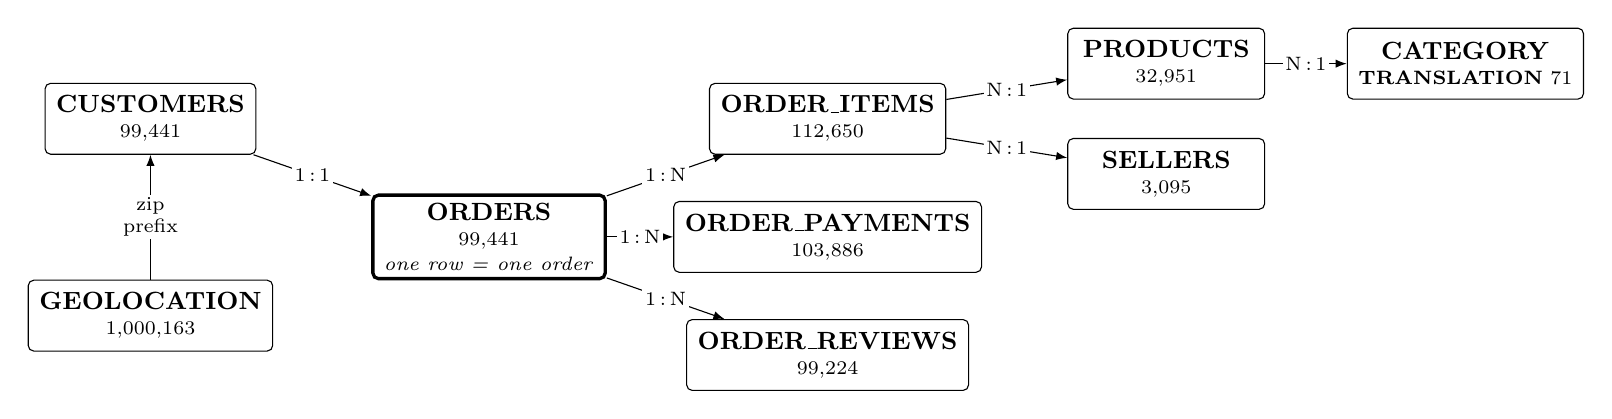
\begin{tikzpicture}[
  font=\small,
  box/.style={draw, rounded corners=2pt, minimum height=9mm, minimum width=25mm,
              inner xsep=4pt, inner ysep=3pt, align=center},
  spine/.style={box, very thick},
  link/.style={draw, -{Latex[length=4pt]}, thin},
  lbl/.style={font=\scriptsize, midway, fill=white, inner sep=1pt}
]
\node[spine] (ord) at (0,0) {\textbf{ORDERS}\\[-2pt]\scriptsize 99{,}441\\[-2pt]\scriptsize \textit{one row = one order}};

\node[box] (cus) at (-4.3,1.5) {\textbf{CUSTOMERS}\\[-2pt]\scriptsize 99{,}441};
\node[box] (itm) at (4.3,1.5) {\textbf{ORDER\_ITEMS}\\[-2pt]\scriptsize 112{,}650};
\node[box] (pay) at (4.3,0) {\textbf{ORDER\_PAYMENTS}\\[-2pt]\scriptsize 103{,}886};
\node[box] (rev) at (4.3,-1.5) {\textbf{ORDER\_REVIEWS}\\[-2pt]\scriptsize 99{,}224};

\node[box] (prd) at (8.6,2.2) {\textbf{PRODUCTS}\\[-2pt]\scriptsize 32{,}951};
\node[box] (sel) at (8.6,0.8) {\textbf{SELLERS}\\[-2pt]\scriptsize 3{,}095};
\node[box] (cat) at (12.4,2.2) {\textbf{CATEGORY}\\[-2pt]\scriptsize \textbf{TRANSLATION} 71};
\node[box] (geo) at (-4.3,-1.0) {\textbf{GEOLOCATION}\\[-2pt]\scriptsize 1{,}000{,}163};

\draw[link] (cus) -- node[lbl]{1\,:\,1} (ord);
\draw[link] (ord) -- node[lbl]{1\,:\,N} (itm);
\draw[link] (ord) -- node[lbl]{1\,:\,N} (pay);
\draw[link] (ord) -- node[lbl]{1\,:\,N} (rev);
\draw[link] (itm) -- node[lbl]{N\,:\,1} (prd);
\draw[link] (itm) -- node[lbl]{N\,:\,1} (sel);
\draw[link] (prd) -- node[lbl]{N\,:\,1} (cat);
\draw[link] (geo) -- node[lbl,align=center]{zip\\prefix} (cus);
\end{tikzpicture}}
\caption{The nine source tables. \code{ORDERS} is the analysis grain. The three
one-to-many children (bold arrows to items, payments and reviews) are each
aggregated to one row per order \emph{before} joining; merging them directly
inflates the table by 19\% and biases every average.}
\label{fig:datamodel}
\end{figure}

\begin{table}[htbp]
\centering
\caption{Data quality audit and cleaning decisions, implemented as
\code{CLEANING\_DECISIONS} in the data-loading module.}
\label{tab:quality}
\small
\begin{tabular}{@{}p{2.7cm}p{4.7cm}p{6.3cm}@{}}
\toprule
\textbf{Issue} & \textbf{Evidence} & \textbf{Decision} \\
\midrule
One-to-many joins &
112{,}650 items and 103{,}886 payments against 99{,}441 orders; a naive merge
yields 118{,}437 rows &
Aggregate each child table to one row per order, then join; assert the grain \\[3pt]

Customer key &
99{,}441 \code{customer\_id} values but 96{,}096 \code{customer\_unique\_id};
2{,}997 people ordered more than once &
Carry \code{customer\_unique\_id} and group on it for repeat behaviour and for
splitting \\[3pt]

Undelivered orders &
2.98\% of orders have no delivery timestamp; status is \emph{delivered} for
97.0\% &
Delivery targets computed only for delivered orders; the rest are \code{NaN},
never imputed \\[3pt]

Review keys &
\code{review\_id} is not unique (789 ids reused); 547 orders carry 2--3 reviews
and 768 carry none &
Key on \code{order\_id}, keep the earliest review; no review means \code{NaN} \\[3pt]

Sparse review text &
\code{review\_comment\_title} present for 11.7\% of reviews,
\code{review\_comment\_message} for 41.3\% &
Use \code{review\_score} only; coverage does not support NLP features \\[3pt]

Geolocation grain &
1{,}000{,}163 rows for 19{,}010 zip prefixes, including points outside Brazil &
Collapse to a median coordinate per prefix; use it for great-circle distance \\[3pt]

Missing product attributes &
610 products (1.9\%) have no category &
Label \code{unknown} rather than dropping orders; impute numerics in-pipeline \\[3pt]

Coverage ramp &
326 orders before 2017; final weeks truncated mid-cycle &
Restrict to 2017-01-01 .. 2018-08-31 (99{,}091 orders) \\[3pt]

Portuguese categories &
71 category names &
Translate to English for all output; keep the original key \\
\bottomrule
\end{tabular}
\end{table}

\begin{table}[htbp]
\centering
\caption{Candidate problems against the brief's scoping checklist.}
\label{tab:checklist}
\small
\begin{tabular}{@{}p{2.5cm}p{4.1cm}p{3.6cm}p{3.5cm}@{}}
\toprule
\textbf{Criterion} & \textbf{C1 delivery (checkout)} & \textbf{C2 low review (delivery)} & \textbf{C3 repeat (checkout)} \\
\midrule
Derivable target & Yes, from order timestamps & Yes, \code{review\_score} $\le 2$ & Yes, next order by person \\
No leakage & Yes, checkout regime & Yes, at-delivery regime & Yes, checkout regime \\
Sufficient signal & Regression yes ($-41\%$ MAE); classification weak (1.6$\times$) & Yes, PR-AUC 0.40 vs 0.11 (3.6$\times$) & No, 2.0$\times$ at a 1.7\% base rate \\
Manageable imbalance & 8.1\% late; loss weights and PR-AUC, no resampling & 14.6\% low; same handling & 2.6\%, too extreme \\
Clear stakeholder & Operations & Customer experience & CRM \\
\midrule
\textbf{Verdict} & \textbf{Primary} & \textbf{Secondary} & Rejected \\
\bottomrule
\end{tabular}
\end{table}

\begin{table}[htbp]
\centering
\caption{Data dictionary for the nine source tables, in the column-level format
used by the NIBRS reference dictionary supplied with the brief. \emph{Nullable}
is measured, not declared: Y means the column actually contains missing values
in this extract, with the observed rate given.}
\label{tab:dictionary}
\scriptsize
\setlength{\tabcolsep}{3.5pt}
% \code forces \small, which is larger than the \scriptsize of this table and
% makes the identifier columns collide. Inside the table, follow the ambient size.
\renewcommand{\code}[1]{\texttt{#1}}
\begin{tabular}{@{}p{2.05cm}p{4.5cm}p{1.15cm}p{1.05cm}p{5.75cm}@{}}
\toprule
\textbf{Table} & \textbf{Column} & \textbf{Type} & \textbf{Null} & \textbf{Comment} \\
\midrule
\code{orders} & \code{order\_id} & text & N & Primary key. The analysis grain \\
 & \code{customer\_id} & text & N & \textbf{Per-order} key, not a person \\
 & \code{order\_status} & text & N & 8 values; \emph{delivered} for 97.0\% \\
 & \code{order\_purchase\_timestamp} & datetime & N & The checkout prediction moment \\
 & \code{order\_approved\_at} & datetime & Y 0.16\% & Post-checkout; excluded as a feature \\
 & \code{order\_delivered\_carrier\_date} & datetime & Y 1.79\% & Post-outcome \\
 & \code{order\_delivered\_customer\_date} & datetime & Y 2.98\% & Post-outcome; defines both delivery targets \\
 & \code{order\_estimated\_delivery\_date} & date & N & Promised at checkout; \textbf{admissible}. Date only, 459 distinct values \\
\midrule
\code{order\_items} & \code{order\_id} & text & N & \textbf{1:N} --- 112,650 rows for 98,666 orders \\
 & \code{order\_item\_id} & int & N & Sequence within the order, 1--21 \\
 & \code{product\_id}, \code{seller\_id} & text & N & Foreign keys \\
 & \code{shipping\_limit\_date} & datetime & N & Post-checkout; excluded \\
 & \code{price}, \code{freight\_value} & float & N & Per item; summed to order level \\
\midrule
\code{order\_payments} & \code{order\_id} & text & N & \textbf{1:N}. One order has no payment row \\
 & \code{payment\_sequential} & int & N & 1--29 \\
 & \code{payment\_type} & text & N & 5 values; credit card 75.4\% \\
 & \code{payment\_installments} & int & N & 0--24; $>1$ for 51.4\% of orders \\
 & \code{payment\_value} & float & N & Summed to order level \\
\midrule
\code{order\_reviews} & \code{review\_id} & text & N & \textbf{Not unique} --- 789 ids reused across orders \\
 & \code{order\_id} & text & N & \textbf{1:N}; 547 orders carry 2--3 reviews \\
 & \code{review\_score} & int & N & 1--5; target of Candidate 2 \\
 & \code{review\_comment\_title} & text & Y 88.3\% & Too sparse to use \\
 & \code{review\_comment\_message} & text & Y 58.7\% & Too sparse to use; no NLP features \\
 & \code{review\_creation\_date} & date & N & Post-outcome for the review target \\
 & \code{review\_answer\_timestamp} & datetime & N & Post-outcome \\
\midrule
\code{customers} & \code{customer\_id} & text & N & Joins 1:1 to orders \\
 & \code{customer\_unique\_id} & text & N & \textbf{The actual person}; 96,096 of them. Grouping key for splits \\
 & \code{customer\_zip\_code\_prefix} & int & N & Joins to geolocation \\
 & \code{customer\_city}, \code{customer\_state} & text & N & 4,119 cities, 27 states \\
\midrule
\code{sellers} & \code{seller\_id} & text & N & 3,095 sellers \\
 & \code{seller\_zip\_code\_prefix} & int & N & Joins to geolocation \\
 & \code{seller\_city}, \code{seller\_state} & text & N & 59.7\% of sellers are in SP \\
\midrule
\code{products} & \code{product\_id} & text & N & 32,951 products \\
 & \code{product\_category\_name} & text & Y 1.85\% & Portuguese; 73 values. Nulls labelled \emph{unknown} \\
 & \code{product\_weight\_g} & float & Y 0.01\% & Summed to order level \\
 & \code{product\_length/height/width\_cm} & float & Y 0.01\% & Combined into item volume \\
 & \code{product\_photos\_qty} & float & Y 1.85\% & Listing-quality proxy \\
\midrule
\code{geolocation} & \code{geolocation\_zip\_code\_prefix} & int & N & 19,015 prefixes over 1,000,163 rows \\
 & \code{geolocation\_lat}, \code{\_lng} & float & N & Collapsed to a median per prefix; out-of-Brazil points dropped \\
\midrule
\code{category\_} & \code{product\_category\_name} & text & N & Join key \\
\code{translation} & \code{product\_category\_name\_english} & text & N & 71 translations \\
\midrule
\multicolumn{5}{@{}l@{}}{\textit{Derived in \code{src/} --- not present in any source file:}} \\
derived & \code{delivery\_days} & float & Y & Purchase to arrival; target of C1A \\
derived & \code{is\_late} & bool & Y & Arrival after the promised date; target of C1B \\
derived & \code{distance\_km} & float & Y 1.2\% & Great-circle customer--seller distance \\
derived & \code{estimated\_days} & float & N & Promised window in days \\
derived & \code{lead\_category} & text & N & Category of the most expensive item \\
derived & \code{freight\_ratio} & float & Y & Freight as a share of item value \\
\bottomrule
\end{tabular}
\end{table}

\newpage
\section{Figures}
\label{app:figures}

\begin{figure}[htbp]
  \centering
  \includegraphics[width=\linewidth]{fig01_coverage_quality.pdf}
  \caption{(a) Monthly order volume. The pilot period before 2017 contributes 326
  orders in total and is excluded from the analysis window. (b) Missingness by
  column: structural rather than random, dominated by orders that never reached
  the customer.}
  \label{fig:coverage}
\end{figure}

\begin{figure}[htbp]
  \centering
  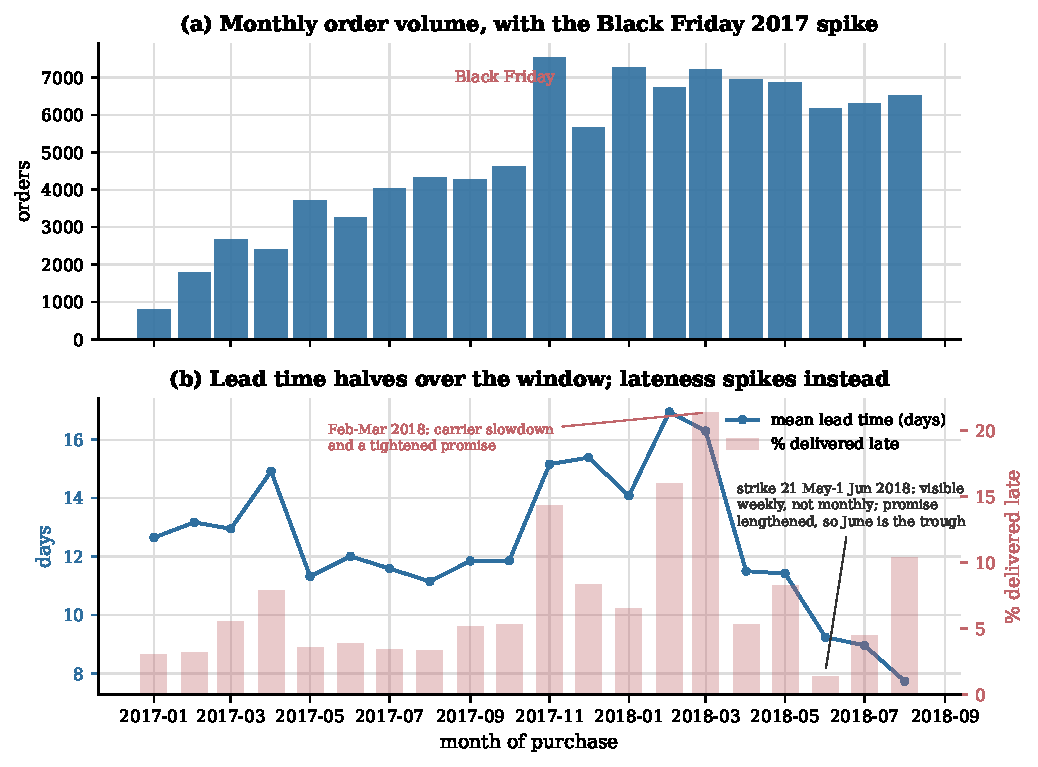
\includegraphics[width=\linewidth]{fig02_volume_drift.pdf}
  \caption{(a) Order volume with the Black Friday 2017 spike. (b) The central
  temporal finding: mean delivery lead time halves across the window (line, left
  axis) while the late rate is volatile rather than trending (bars, right axis),
  spiking at Black Friday and during the May 2018 truckers' strike.}
  \label{fig:volume}
\end{figure}

\begin{figure}[htbp]
  \centering
  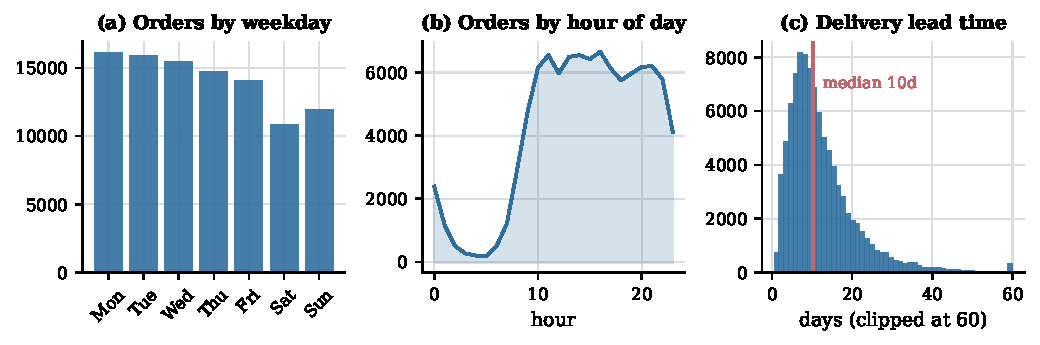
\includegraphics[width=\linewidth]{fig03_rhythm.pdf}
  \caption{Purchase rhythm and the lead-time distribution. Ordering is
  weekday-heavy and peaks at 16:00; lead time is right-skewed with a median of
  10.2 days and a long tail.}
  \label{fig:rhythm}
\end{figure}

\begin{figure}[htbp]
  \centering
  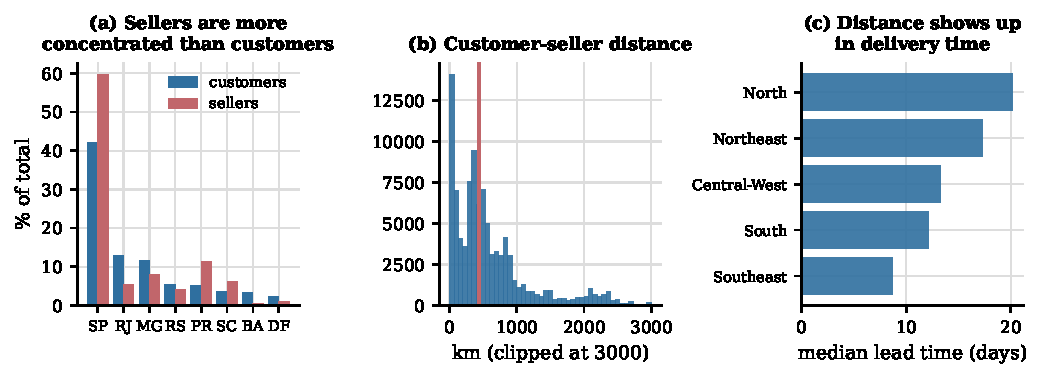
\includegraphics[width=\linewidth]{fig04_geography.pdf}
  \caption{(a) Sellers are far more concentrated in S\~{a}o Paulo than customers
  are, so most orders must cross the country. (b) Customer--seller distance.
  (c) That distance shows up directly in regional delivery times.}
  \label{fig:geography}
\end{figure}

\begin{figure}[htbp]
  \centering
  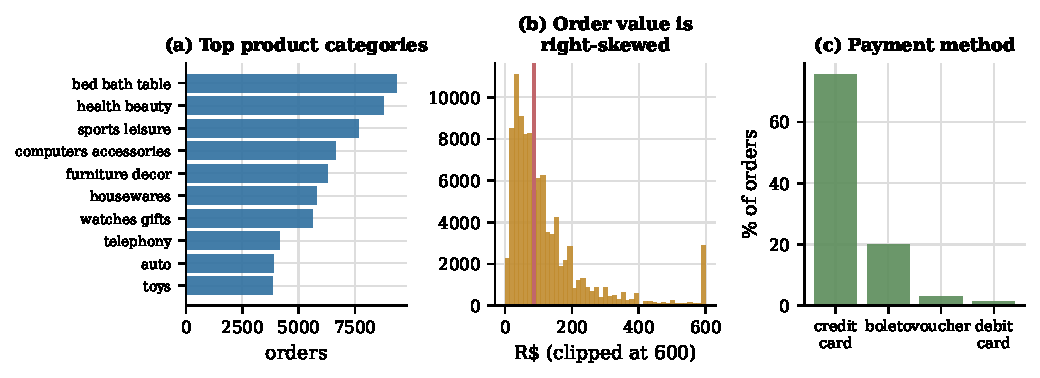
\includegraphics[width=\linewidth]{fig05_products_money.pdf}
  \caption{(a) Demand is long-tailed across 74 categories. (b) Order value is
  strongly right-skewed. (c) Credit card dominates, usually in instalments.}
  \label{fig:products}
\end{figure}

\begin{figure}[htbp]
  \centering
  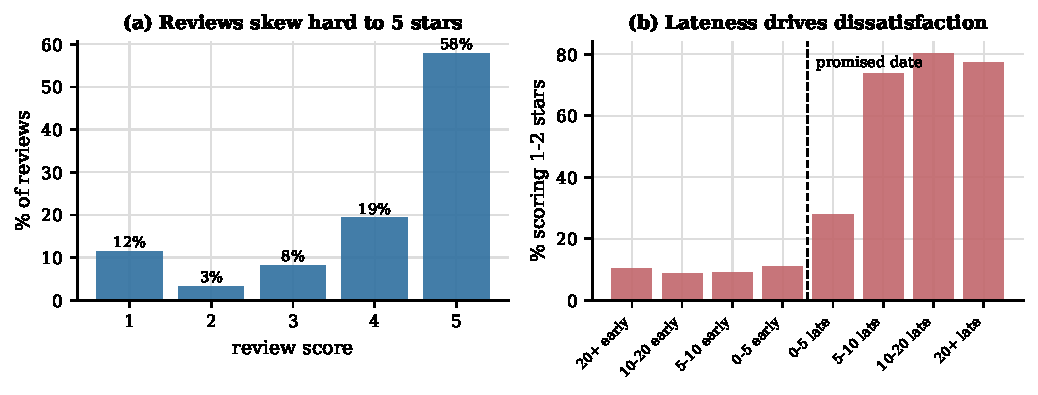
\includegraphics[width=\linewidth]{fig06_reviews_delivery.pdf}
  \caption{(a) Reviews are severely imbalanced towards five stars. (b) The
  strongest relationship in the dataset: the 1--2 star rate rises monotonically
  with lateness, from 9.2\% for on-time orders to 54.0\% for late ones.}
  \label{fig:reviews}
\end{figure}

\begin{figure}[htbp]
  \centering
  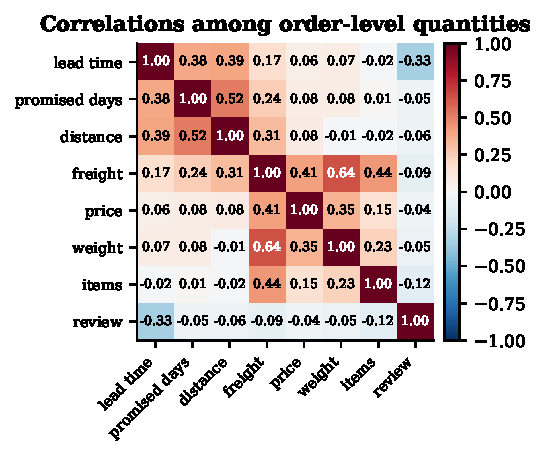
\includegraphics[width=0.62\linewidth]{fig07_correlations.pdf}
  \caption{Correlations among order-level quantities. Distance and the platform's
  own promise are the strongest checkout-time correlates of lead time.}
  \label{fig:correlations}
\end{figure}

\begin{figure}[htbp]
  \centering
  \includegraphics[width=0.58\linewidth]{fig08_leakage.pdf}
  \caption{What one forbidden column is worth. Adding the realised delivery time
  to the late-delivery model takes ROC-AUC from 0.589 to 1.000 --- the model is
  reading the answer, not predicting it.}
  \label{fig:leakage}
\end{figure}

\begin{figure}[htbp]
  \centering
  \includegraphics[width=\linewidth]{fig09_candidates.pdf}
  \caption{Candidate comparison. (a) PR-AUC against the no-skill floor for each
  candidate and prediction moment. (b) Lead-time MAE: the platform's own promise
  is worse than a constant. (c) Raw accuracy flatters every imbalanced target;
  balanced accuracy does not.}
  \label{fig:candidates}
\end{figure}

% ============================== AI DECLARATION =============================
\clearpage
\section*{AI Tool Declaration}
\addcontentsline{toc}{section}{AI Tool Declaration}

We used OpenAI's ChatGPT and Anthropic's Claude to generate and validate ideas,
improve expression and refine our writing. We also used the models to debug our
code. All analytical decisions, results and conclusions were reviewed and
verified by the team against the underlying data, and we are responsible for the
content and quality of the submitted work.

\end{document}
